\begin{wrapfigure}{r}{0.5\textwidth}
	\centering
	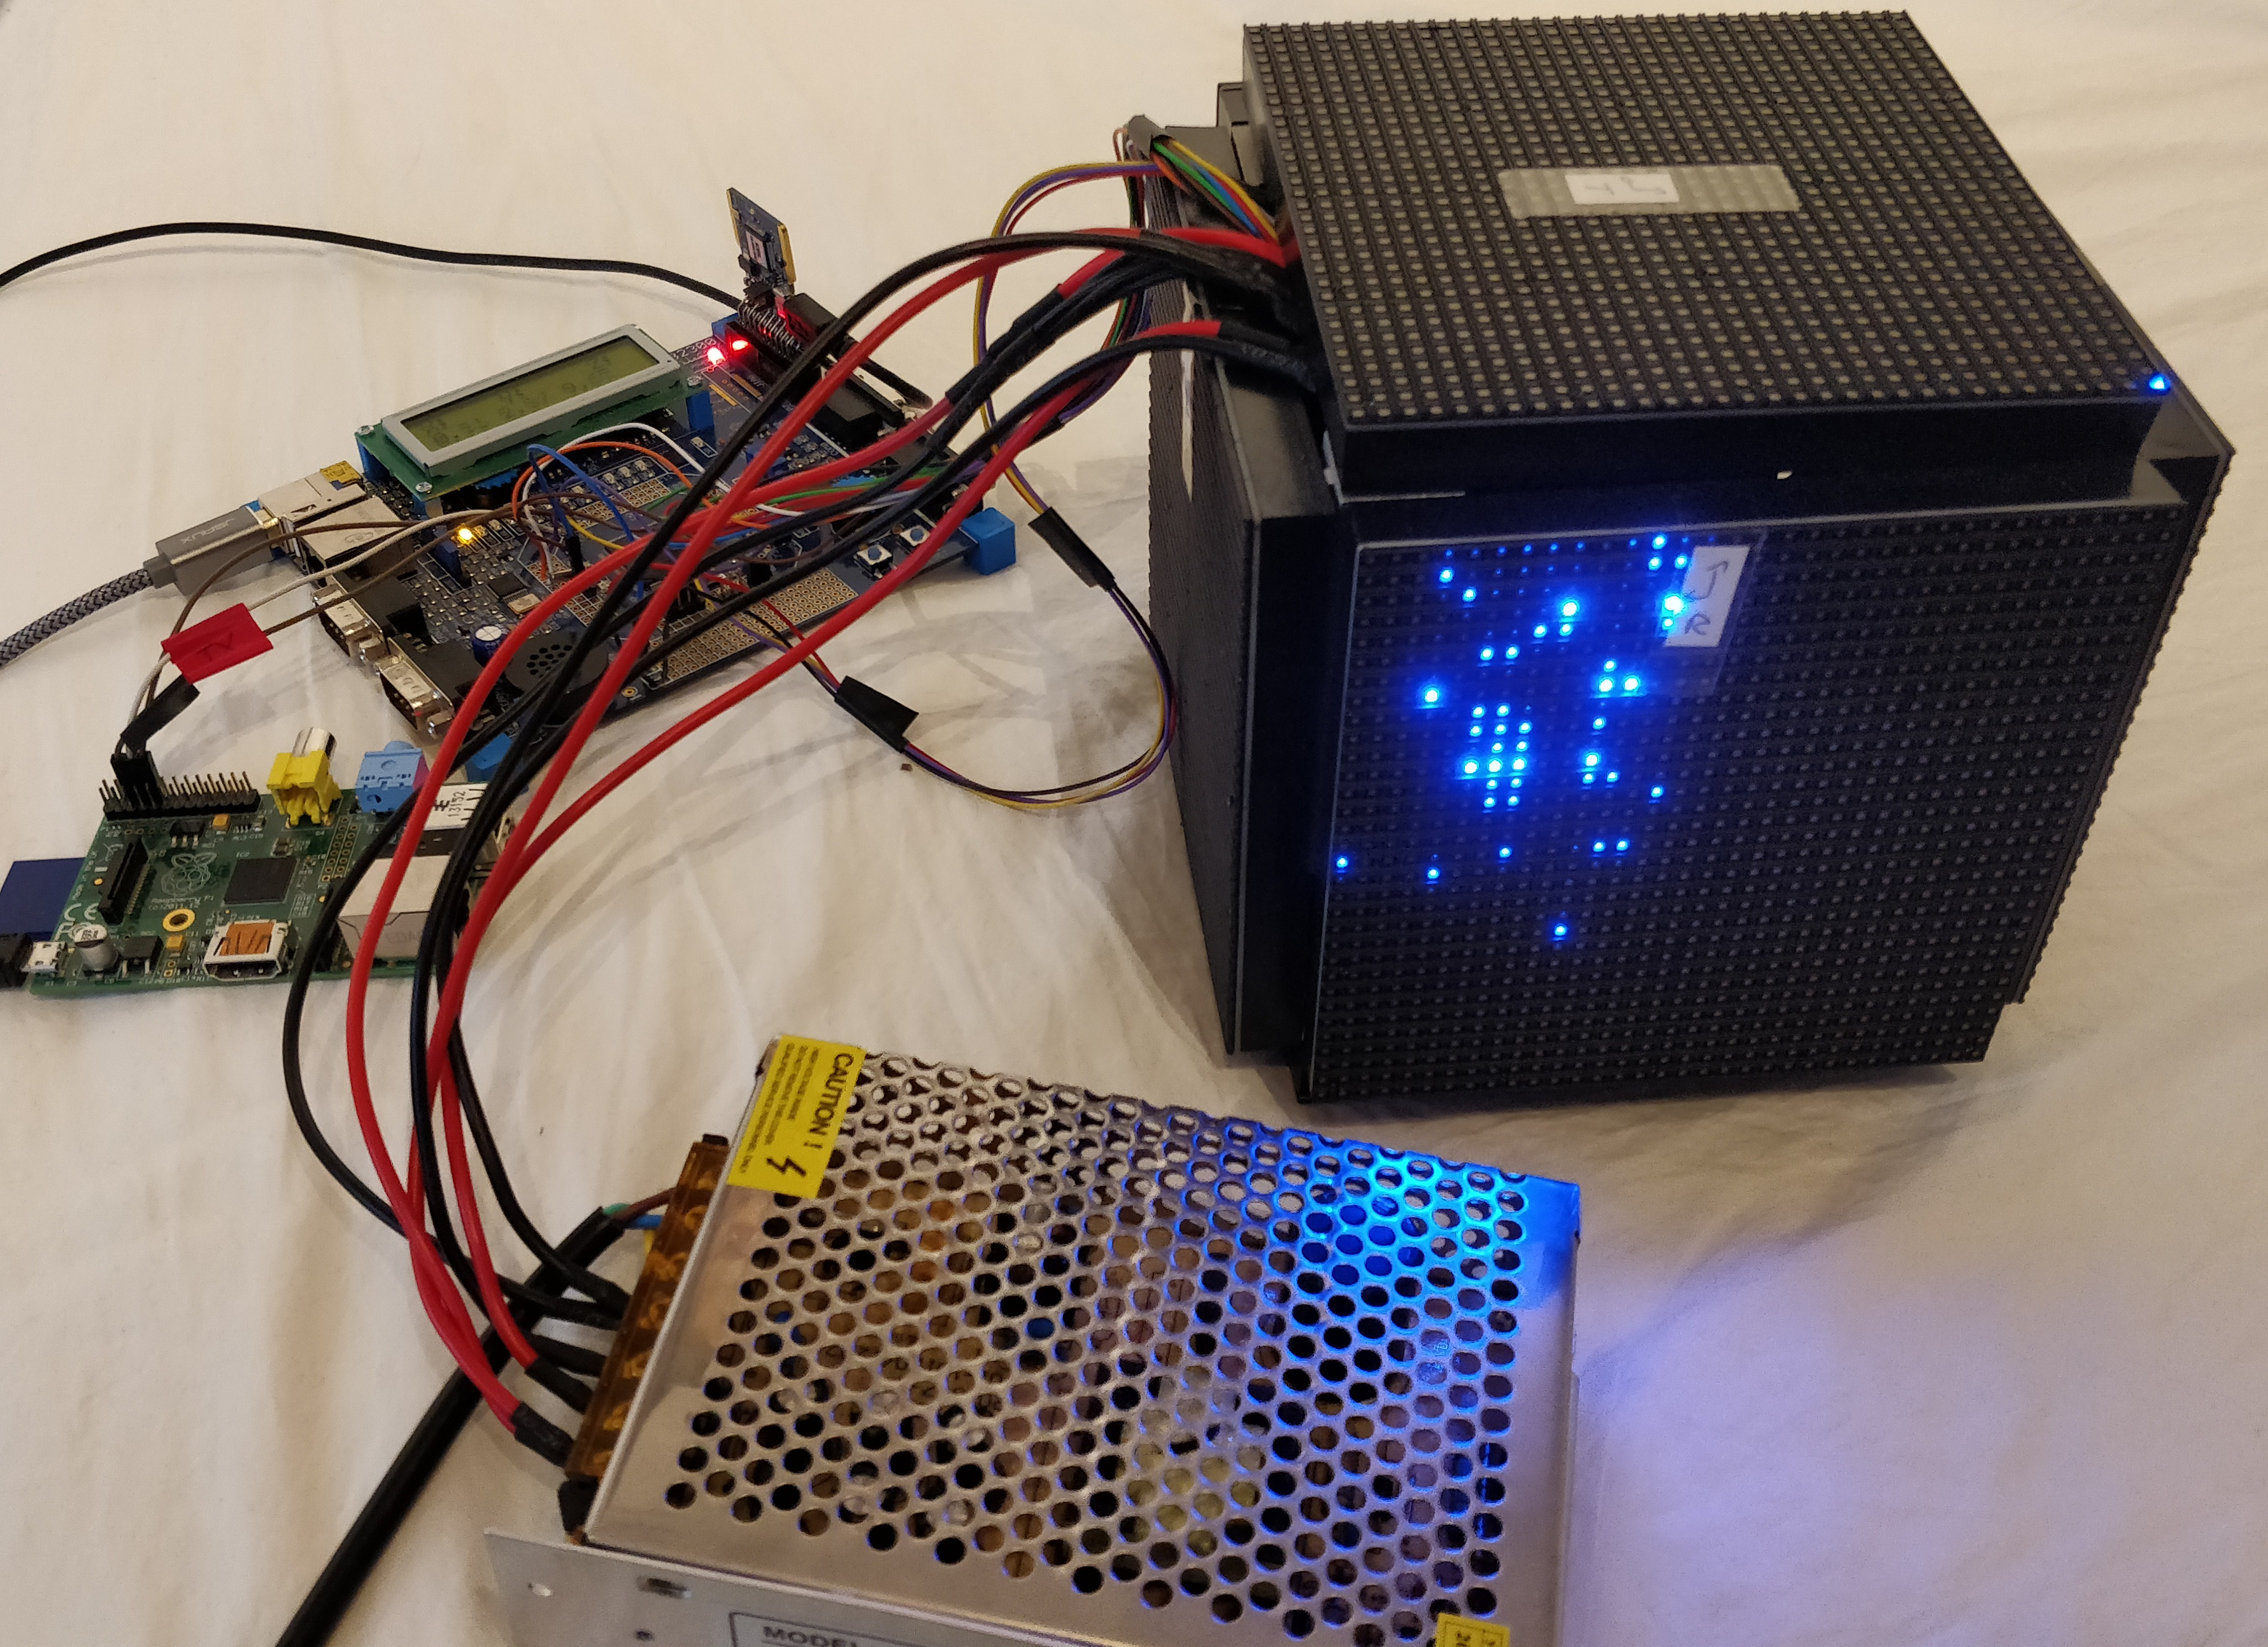
\includegraphics[width=.45\textwidth]{IMG_20190411_030828.jpg}
	\caption{Fertiger Aufbau}
	\label{fig:result}
\end{wrapfigure}

Im Verlaufe des Projektes konnte erfolgreich eine einfache Flüssigkeitssimulation implementiert werden, welche auf unterschiedlichen Plattformen ausgeführt werden kann (getestet: Linux, ARM none). Die Simulation ist einfach skalierbar mit mehr Partikeln oder anderen Displaymaßen. Die Grundlagen einer Ausgelagerten Berechnung der Pixeldaten und der Kommunikation via UART zwischen einem Raspberry Pi 1B und dem \texttt{LPC2388} wurden geschaffen, die Fertigstellung scheiterte jedoch an Fehlern im Interruptmanagement der Geräte. Auf Grund der schwierigen Dokumentationslage beim \texttt{Raspberry Pi} ist dies jedoch sehr zeitaufwendig. Erfolgreich ist das Senden der Daten des Beschleunigungssensors, sowie er Pixeldaten vom\texttt{Raspberry Pi}, welcher wie der \texttt{LPC2388} ohne Betriebssystem programmiert worden ist.

Ebenso haben wir, via SPI, den \texttt{AXL345} Beschleunigungssensor angebunden und dessen Orientierung ausgelesen. Diese Daten fließen in die Simulation mit ein. Die Ansteuerung der LED-Panele mit $24$Bit Farbauflösung ist ebenso erfolgreich implementiert worden und kann auf beliebig viele weitere Displays beliebiger Seitenmaße erweitert werden.